\lab{Complex Integration}{Integration in the Complex Plane}{Integration in the Complex Plane}

\objective{Understand some simple uses of residues and singularities in the complex plane.}

In Lab \ref{Lab:complex_intro} we demonstrated the fact that integrals of holomorphic functions are independent of path.
Here we will consider the effect that singularities have on this property.

\section*{Residues}

We will now introduce another form of series representation of functions.
A Laurent series of a function is a series of the form
\[\sum_{n= -\infty}^{\infty} a_n (z-z_0)^n\]
It can be proven that
\[a_n = \frac{1}{2\pi i} \int_C \frac{f(z)}{(z-z_0)^{n+1}} dz\]
Where $C$ is a contour which passes counterclockwise around the singularity exactly once.
When $f$ does not have a singularity at $z_0$ this representation degenerates to a normal Taylor Series (with the derivatives evaluated by the formula for the $n$th derivative of an analytic function).
These sorts of series are considered in greater detail in the text.
The built in function \li{sympy.series} can evaluate the series expansion of a function at a singularity, for example
\begin{lstlisting}
import sympy as sy
z = sy.Symbol('z')
(1/sy.sin(z)).series(z,0,8)
\end{lstlisting}

The Laurent series representation provides a simple way to classify singularities in the complex plane.
Isolated singular points can be classified as removable singular points, poles, or essential singular points.
These definitions will also be discussed in greater detail in the text.
Here we will show one method for visualizing complex functions around singular points.
In Lab \ref{Lab:complex_intro} we presented surface plots as a useful method for visualizing well-behaved functions in the complex plane.
Here we will also show how to use surface and color plots to visualize complex functions near their poles.

To make a surface plot about a singularity, we must account for the fact that the function is not going to be defined at all of the points we use in our graph.
We will also have to limit the $z$ axis on the plot to avoid creating a plot that is dominated exclusively by the extremely large and extremely small values in of the function.
Plotting libraries like Mayavi and Matplotlib do allow thresholding of 3D plots via the use of floating point values of \li{nan}, but doing this may result in graphs having jagged edges where they have been cut.
We can avoid the jagged edges by artificially adding a small lip of constant values to the plot as well.
This can be done with Matplotlib as follows:
\begin{lstlisting}
mn, mx = -1, 1
res = 401
lip = 2.
tol = 100
x = np.linspace(mn, mx, res)
X, Y = np.meshgrid(x, x, copy=False)
Z = 1 / (X + 1.0j * Y)
Z = Z.real
Z[(threshold+lip>Z)&(Z>threshold)] = threshold
Z[(-threshold-lip<Z)&(Z<-threshold)] = -threshold
Z[np.absolute(Z) >= threshold + lip] = np.nan
fig = plt.figure()
ax = fig.gca(projection='3d')
ax.plot_surface(X, Y, Z)
plt.show()
\end{lstlisting}

Figures \ref{fig:inv_surfaces} %and \ref{fig:inv2_surfaces} show surface plots of some relatively well-behaved singular points.

\begin{figure}
\begin{subfigure}{.32\textwidth}
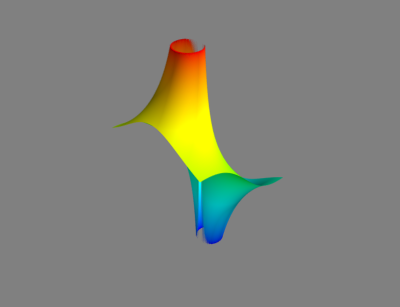
\includegraphics[width=\textwidth]{inv_real_surface.png}
\end{subfigure}
\begin{subfigure}{.32\textwidth}
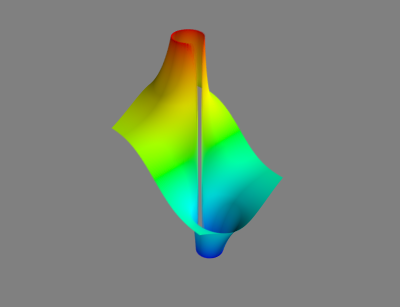
\includegraphics[width=\textwidth]{inv_imag_surface.png}
\end{subfigure}
\begin{subfigure}{.32\textwidth}
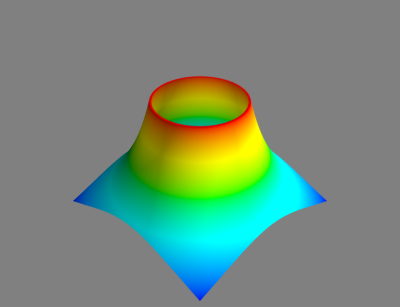
\includegraphics[width=\textwidth]{inv_abs_surface.png}
\end{subfigure}
\caption{Surface plots of the real part, imaginary part, and absolute value of $\frac{1}{z}$ about the origin.}
\label{fig:inv_surfaces}
\end{figure}

\begin{figure}
\begin{subfigure}{.32\textwidth}
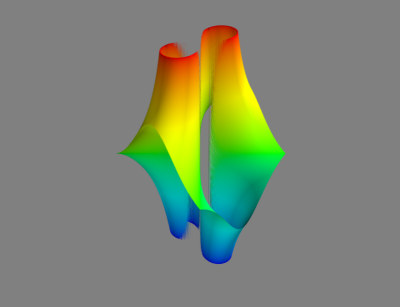
\includegraphics[width=\textwidth]{inv2_real_surface.png}
\end{subfigure}
\begin{subfigure}{.32\textwidth}
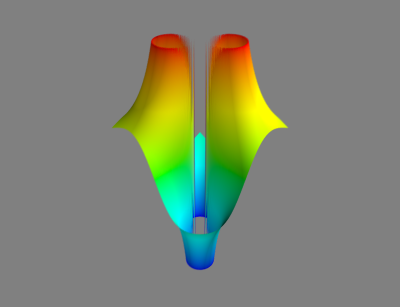
\includegraphics[width=\textwidth]{inv2_imag_surface.png}
\end{subfigure}
\begin{subfigure}{.32\textwidth}
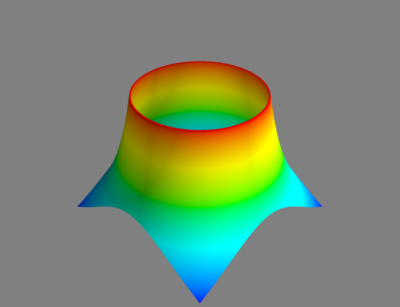
\includegraphics[width=\textwidth]{inv2_abs_surface.png}
\end{subfigure}
\caption{Surface plots of the real part, imaginary part, and absolute value of $\frac{1}{z}$ about the origin.}
\label{fig:inv2_surfaces}
\end{figure}

Color plots, when used in their default form suffer from similar limitations.
On the other hand, we can do things like taking the absolute value, then scaling the values of a function logarithmically to mitigate some of the effect that the rapid growth of the plot values has on the colors in the plot.
We can also allow the color map used by the plotting library to repeat itself as the values of the function get larger and larger.
This can be done by taking the sine of the values.
Combining these things together, we obtain expressions like $\sin\left(\log\left|\text{Re}\left(Z\right)\right|\right)$.
Figures \ref{fig:inv_color}, \ref{fig:inv4_color}, \ref{fig:exp_inv_color}, and \ref{fig:exp_inv2_color} all show color plots that have been generated using this approach.
This is one of a variety of ways to produce color plots that represent complex valued functions.

\begin{figure}
\begin{subfigure}{.32\textwidth}
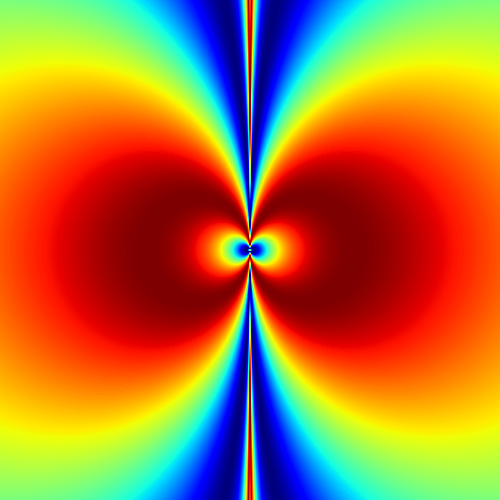
\includegraphics[width=\textwidth]{inv_real.png}
\end{subfigure}
\begin{subfigure}{.32\textwidth}
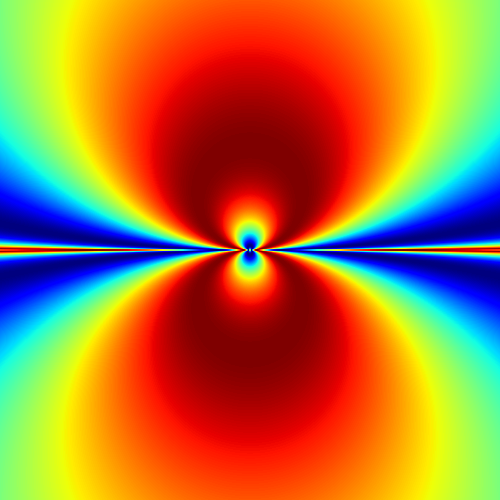
\includegraphics[width=\textwidth]{inv_imag.png}
\end{subfigure}
\begin{subfigure}{.32\textwidth}
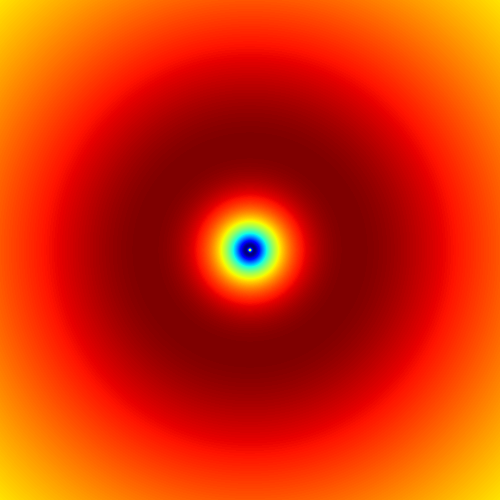
\includegraphics[width=\textwidth]{inv_abs.png}
\end{subfigure}
\caption{Color plot representations of the real part, imaginary part, and absolute value of $\frac{1}{z}$ about the origin.}
\label{fig:inv_color}
\end{figure}

\begin{figure}
\begin{subfigure}{.32\textwidth}
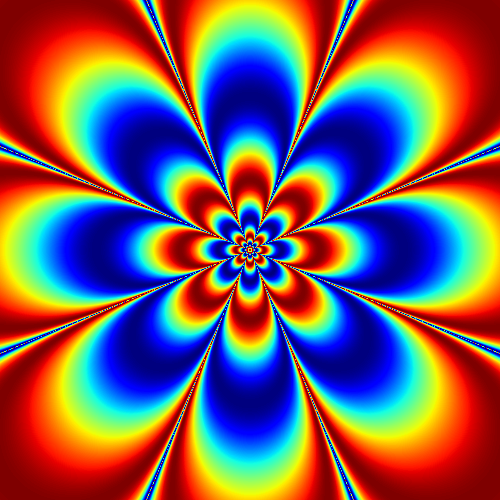
\includegraphics[width=\textwidth]{inv4_real.png}
\end{subfigure}
\begin{subfigure}{.32\textwidth}
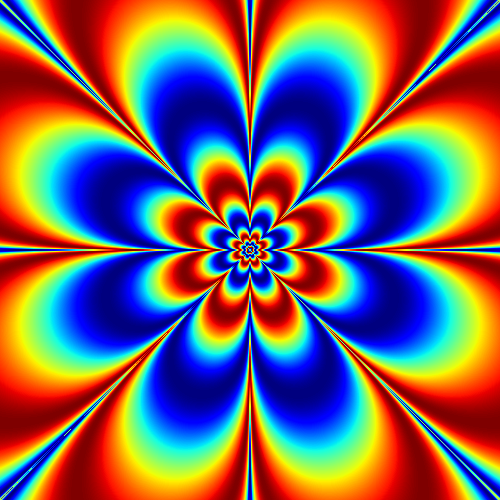
\includegraphics[width=\textwidth]{inv4_imag.png}
\end{subfigure}
\begin{subfigure}{.32\textwidth}
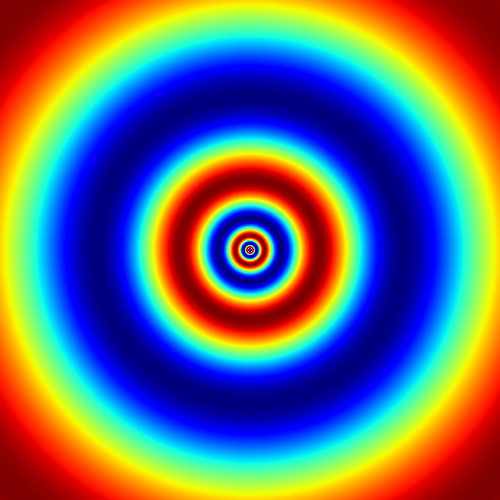
\includegraphics[width=\textwidth]{inv4_abs.png}
\end{subfigure}
\caption{Color plot representations of the real part, imaginary part, and absolute value of $\frac{1}{z^4}$ about the origin.}
\label{fig:inv4_color}
\end{figure}

\begin{figure}
\begin{subfigure}{.32\textwidth}
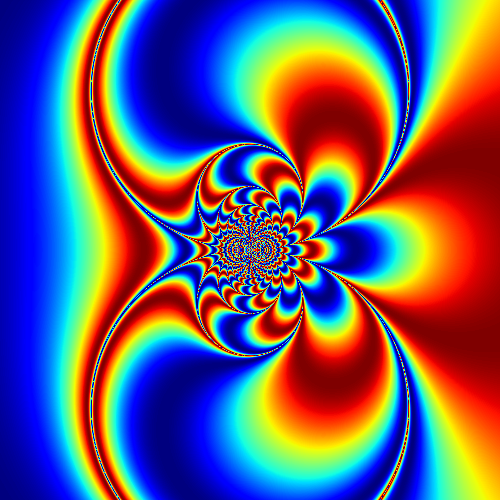
\includegraphics[width=\textwidth]{exp_inv_real.png}
\end{subfigure}
\begin{subfigure}{.32\textwidth}
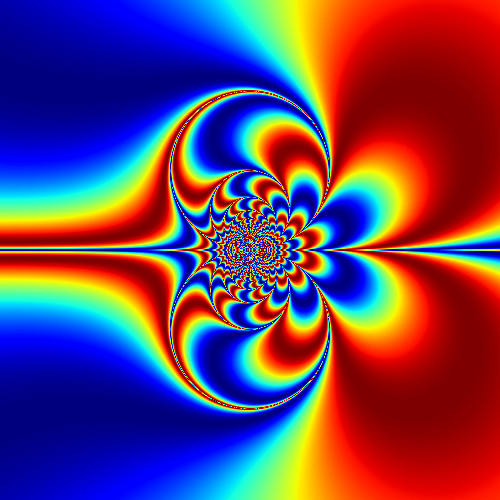
\includegraphics[width=\textwidth]{exp_inv_imag.png}
\end{subfigure}
\begin{subfigure}{.32\textwidth}
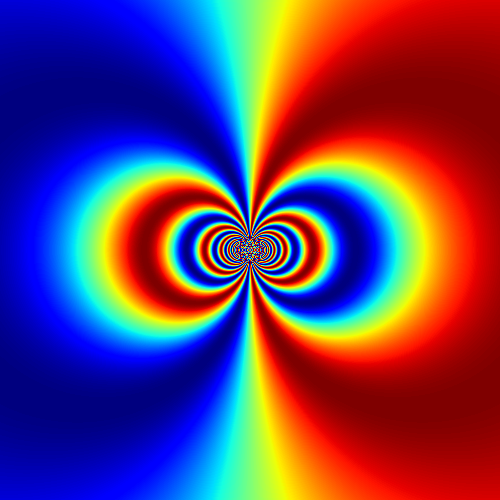
\includegraphics[width=\textwidth]{exp_inv_abs.png}
\end{subfigure}
\caption{Color plot representations of the real part, imaginary part, and absolute value of $e^{\frac{1}{z}}$ about the origin.
This is an essential singular point.}
\label{fig:exp_inv_color}
\end{figure}

\begin{figure}
\begin{subfigure}{.32\textwidth}
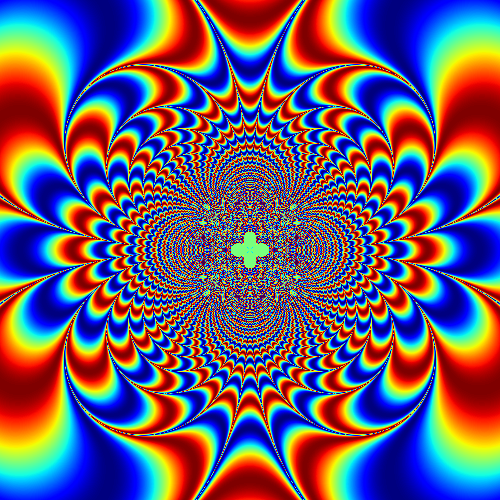
\includegraphics[width=\textwidth]{exp_inv2_real.png}
\end{subfigure}
\begin{subfigure}{.32\textwidth}
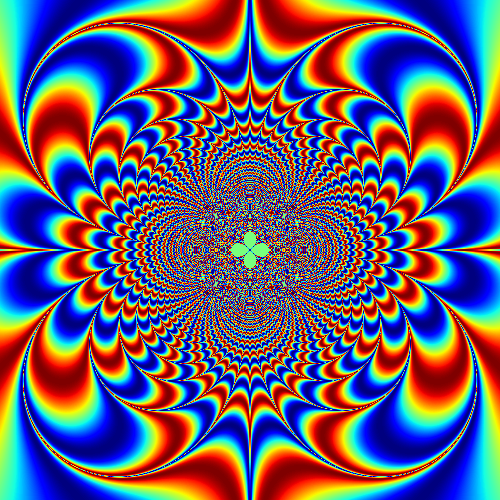
\includegraphics[width=\textwidth]{exp_inv2_imag.png}
\end{subfigure}
\begin{subfigure}{.32\textwidth}
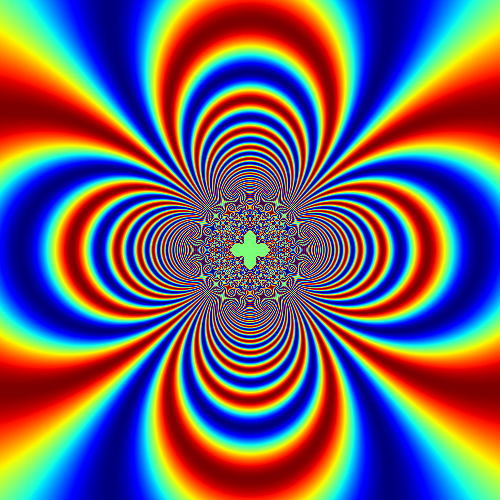
\includegraphics[width=\textwidth]{exp_inv2_abs.png}
\end{subfigure}
\caption{Color plot representations of the real part, imaginary part, and absolute value of $e^{\frac{1}{z^2}}$ about the origin.
This is an essential singular point.}
\label{fig:exp_inv2_color}
\end{figure}

The number $a_{-1}$ in the Laurent expansion for a function $f$ at a point $z_0$ is called the Residue of $f$ at $z_0$.
The formula for the coefficients of the Laurent series provides one way to compute residues.
It is sometimes easier to evaluate a residue using limits.
To see how this might be done, consider some function $f$ with a pole of order $1$ at $z_0$.
We say $f$ has a pole of order $n$ at $z_0$ if the first nonzero term in the Laurent Series expansion of is the term corresponding to $(z-z_0)^{-n}$.
In the case of our pole of order 1, we then have
\[f(z)=c_{-1}(z-z_0)^{-1}+c_0 (z-z_0)^{0} +c_1 (z-z_0) + \dots\]
So,
\[f(z)(z-z_0)=c_{-1}+c_0 (z-z_0) + c_1 (z-z_0)^2 + \dots\]
Since the right hand side of the Laurent series converges within some nonzero distance of $z_0$, this series will also converge on that domain.
It is an ordinary power series, so it will also be continuous on that domain (it will actually be analytic, but continuity is sufficient here).
This means that we may take the limit of this expression as $z$ approaches $z_0$.
Taking this limit, the only nonzero term of the series remaining is $c_{-1}$, so we have
\[\lim_{z\to z_0} f(z)(z-z_0) = c_{-1} = \Res{z=z_0} f(z)\]
Now for some $f(z)$ with a pole of order $n$ at $z_0$ we have that within some nonzero distance of $z_0$, the Laurent series of $f$ converges and is of the form
\[f(z)=c_{-n}(z-z_0)^{-n}+\dots+c_0+c_1(z-z_0)+\dots\]
Multiplying by $(z-z_0)^{n}$ and differentiating $n-1$ times, we have
\[\frac{d^{n-1}}{dz^{n-1}}(f(z)(z-z_0)^{n})=(n-1)! c_{-1} + \frac{n!}{1!} c_0 (z-z_0) + \frac{(n+1)!}{2} c_1 (z-z_0)^2!+\dots\]
Taking the limit, we have
\[\lim_{z\to z_0}\frac{d^{n-1}}{dz^{n-1}}((z-z_0)^n f(z)) = (n-1)! c_{-1}\]
Which implies
\[\Res{z=z_0}f(z)=\frac{1}{(n-1)!}\lim_{z\to z_0}\frac{d^{n-1}}{dz^{n-1}}((z-z_0)^n f(z))\]
Another useful trick involving poles and residues involves the logarithmic residue, i.e. the residue of the logarithmic derivative $\frac{d}{dz}(\ln(f(z))) = \frac{f'(z)}{f(z)}$.
A natural consequence of the Laurent series expansion of $f(z)$ and $f'(z)$ at a pole $z_0$ is that, where $d$ is the degree of the pole at $z_0$ is that
\[- \Res{z=z_0} \frac{f'(z)}{f(z)} = d\]
This is a useful bit of information that may be used to simplify computation of residues or of the Laurent series expansion of a function.
Another way we can evaluate residues is by the following theorem.
\begin{theorem}
Let $f(z)=\frac{p(z)}{q(z)}$ and let $p$ and $q$ be holomorphic at $z_0$. Let $p(z_0) \neq 0$ and $q(z_0)=0$.
Suppose that $z_0$ is a pole of order $1$ of $f$.
Then
\[\Res{z=z_0} f(z) = \frac{p(z_0)}{q'(z_0)}\]
\end{theorem}

\begin{problem}
Write a Python function that given a function and one of it's poles uses \li{sympy.residue} to calculate the order of that pole and with that information calculate the residue of the function using symbolic limits and derivatives.
Verify that your function calculates the correct order and check the residue against \li{sympy.residue}, using the function
\[f(z) = \frac{1}{(z^+1)^{4}(2z+1)}dz\]
(The roots are somewhat obvious here, but as a note you can use \li{sympy.solve} to find the roots).
\end{problem}

\begin{problem}
Write a python function, which, using symbolic integration in SymPy, returns the Laurent series expansion of a function about a given pole.
Use the trick involving logarithmic residues to figure out what the degree of the pole is, then use symbolic limits and derivatives to compute the coefficients of the corresponding Laurent series expansion (look at the original equation for the coefficients of the Laurent Series and see that they can be rewritten as residues).
You may assume that the pole is not an essential singular point.
(Recall that, as we defined it, a pole is not an essential singular point, so it will always have a finite degree).
\end{problem}

\section*{Evaluating Indefinite Integrals Using Residues}

One convenient use of residues is the evaluation of integrals that are difficult to evaluate symbolically in other ways.
Often, when we cannot directly assign a value to one of these integrals, residues can still help us evaluate the Cauchy principal value of the integral.
Recall that for an integral $\int_{-\infty}^{\infty} f(x)dx$ the Cauchy principal value is $\lim_{r\to \infty} \int_{-r}^{r} f(x) dx$.
This limit may exist, even though the limit itself may not.

\begin{figure}
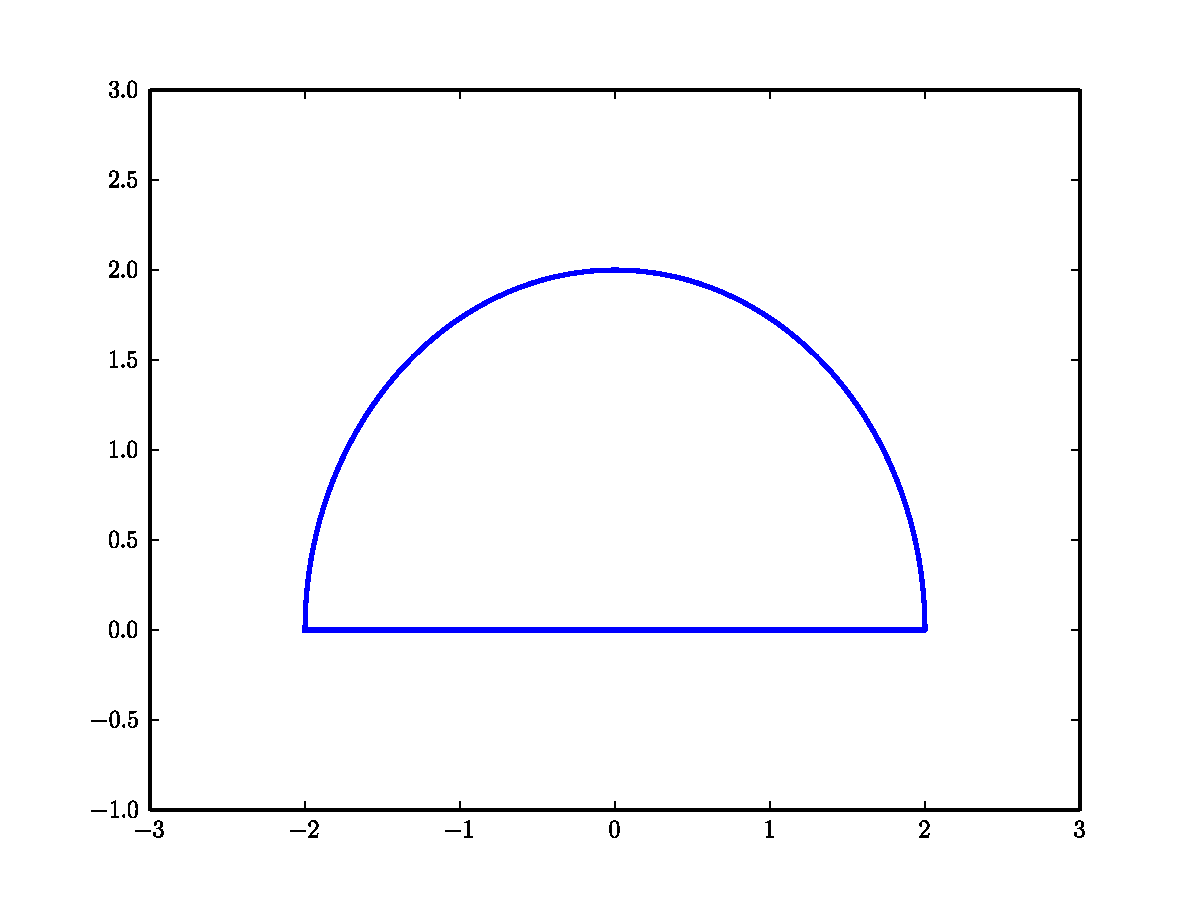
\includegraphics[width=\textwidth]{contour1.pdf}
\caption{A contour used for integration using residues.}
\label{complexint:c1}
\end{figure}

Consider the integral $\int_{-\infty}^{\infty}\frac{z^2}{z^4+1}$. Let $f(z)=\frac{z^2}{z^4+1}$.
Notice that this function has poles at $e^{\frac{\pi i}{4}}$, $e^{\frac{3\pi i}{4}}$, $e^{\frac{5\pi i}{4}}$, and $e^{\frac{7\pi i}{4}}$.
For notation, let these be $p_1$, $p_2$, $p_3$, and $p_4$.
For some real $R>1$, consider the contour $C$ from $-R$ to $R$ and counterclockwise along the circle centered at $0$ of radius $R$ back to -$R$.

This contour ( a semi circle) is shown in Figure \ref{complexint:c1} with $R = 2$.
Let $A$ be this second portion of $C$.
Note that, since $R>1$ we have
\[\int_C f(z)dz = 2\pi i (\Res{z=p_0} f(z) +\Res{z=p_1} f(z))\]
So, rewriting, we have
\[\int_{-R}^R f(z) dz = 2\pi i (\Res{z=p_0} f(z) +\Res{z=p_1} f(z)) - \int_A f(z) dz\]
so
\[\int_{-\infty}^{\infty} f(z) dz = \lim_{R\to \infty} \int_{-R}^R f(z) dz = 2\pi i (\Res{z=p_0} f(z) +\Res{z=p_1} f(z)) - \lim_{R\to \infty} \int_A f(z) dz\]
We would like to show that that $\lim_{R\to\infty} \int_A f(z) dz = 0$, so note that on $A$, $\abs{z}=R$.
It follows from the triangle inequality that $\abs{z^4+1}\geq \abs{\abs{z}^4-1} = R^4 -1$, so we have that
\[\abs{\int_A f(z) dz}\leq \int_A \abs{f(z)} dz \leq \int_A \frac{R^2}{R^4 -1}dz = \pi R \frac{R^2}{R^4-1}\]
so $\lim_{R\to\infty} \int_A f(z) dz = 0$ as desired.
This then implies that
\[\int_{-\infty}^{\infty} f(z) dz = 2\pi i (\Res{z=p_0} f(z) +\Res{z=p_1} f(z))\]
Evaluating the residues at $p_0$ and $p_1$ we have
\[\int_{-\infty}^{\infty} f(z) dz = \frac{\pi}{\sqrt{2}}\]

\begin{problem}
Write a python function which, given the coefficients for the polynomials in the numerator and denominator of a rational function $f$, evaluates the sum
\[\sum 2\pi i (\Res{z=p} f(z))\]
over all poles $p$ of $f$ such that $Im(p)>0$.
Use that function to numerically evaluate the following integrals.
\[\int_{-\infty}^{\infty} \frac{z^2}{z^6+1}dz\]
\[\int_{-\infty}^{\infty} \frac{z^{12}-5z^{10}+3z^8-16z^6+4z^4-z^2-4}{4z^{14}+6z^6+12}dz\]
\end{problem}

\begin{problem}
Similar arguments can be used to evaluate integrals of functions that can be compared to the rational functions in question.
Write a modified version of the function you just wrote and use it to evaluate the following integrals.
\[\int_{-\infty}^{\infty}\frac{cos(z)}{z^4+1}dz\]
\[\int_{-\infty}^{\infty}\frac{sin^2(z)}{z^{20}+1}dz\]
\end{problem}

The general conditions in which we may apply this particular way of evaluating integrals come from Jordan's Lemma, which states
\begin{lemma}[Jordan's Lemma]
If for some $f(z)$ on $\mathbb{C}$, $f$ is analytic for all points $z$ in the upper half plane such that $\abs{z}>R_0$ for some $R_0 \in \mathbb{R}$ where $R_0 >0$ and that, where $C_R$ denotes the semicircle $z=Re^{i\theta}$ for $0\leq \theta \leq \pi$, there exists some positive constant $M_R$ such that for all $z$ on $C_R$, $\abs{f(z)} \leq M_R$ and $\lim_{R \to \infty} M_R = 0$, then for every positive constant $a$, we have
\[\lim_{R \to \infty} \int_{C_R} f(z) e^{iaz} dz = 0\]
\end{lemma}

\begin{problem}
Use the function you just wrote to evaluate the Cauchy Principal Value of the integral
\[\int_{\infty}^{-\infty} \frac{z sin(z)}{z^2+1}\]
\end{problem}

If a function has a singularity on the real line, we can often still evaluate the value of $\int_{-\infty}^{\infty} f(z) dz$ using a similar argument as before, but by indenting the path along the real axis around a small path around the singularity, then, as we take the limit as our outer contour moves out toward infinity, we can let the small contour around the singularity approach the singularity.
An example of a contour like this is shown in Figure \ref{complexint:c2}.
It is centered at the origin with $R=2$ on the outer circle and $R=\frac{1}{2}$ on the inner circle.

\begin{figure}
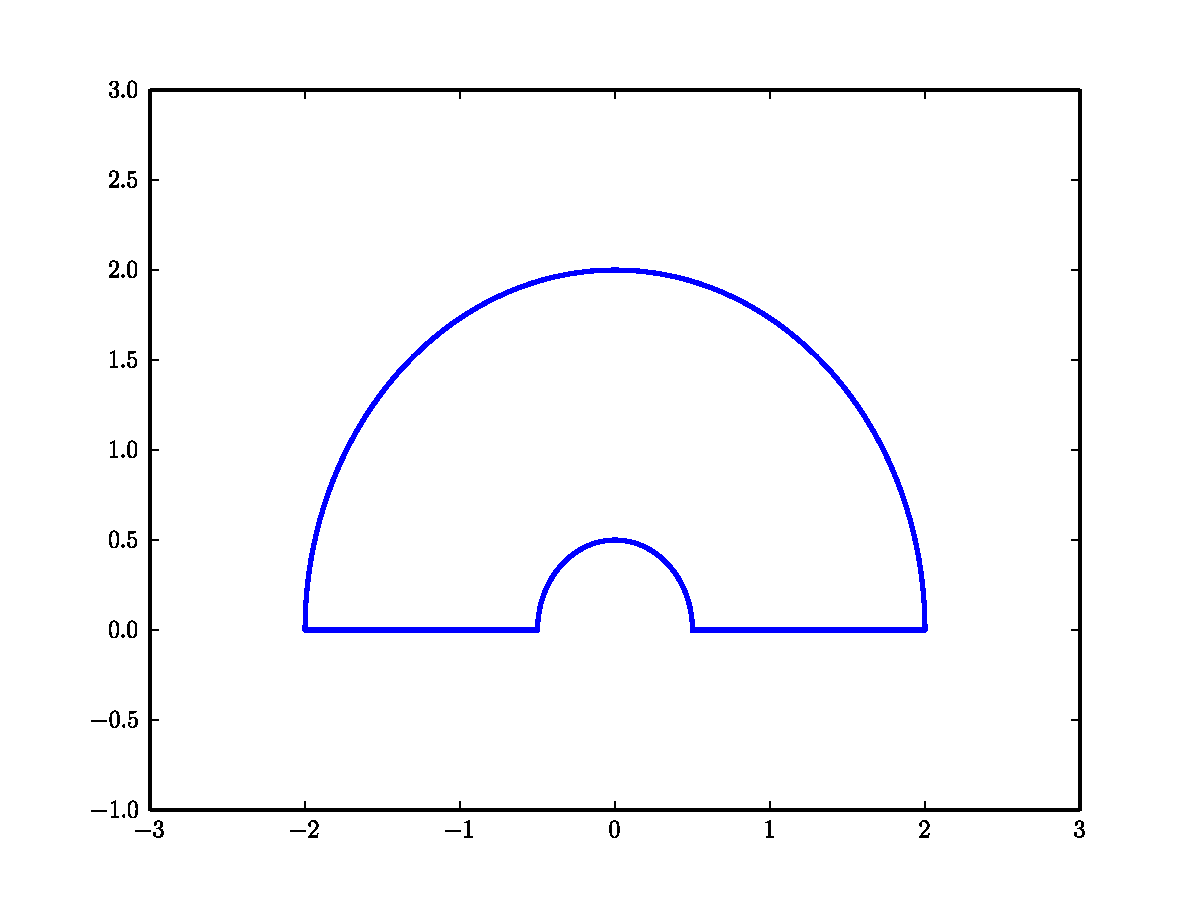
\includegraphics[width=\textwidth]{contour2.pdf}
\caption{An example of a contour that has been modified to avoid a singularity along the real line.}
\label{complexint:c2}
\end{figure}

The following is a useful theorem involving these ``indented path" methods.
\begin{theorem}
Consider a function $f$ with a pole of order $1$ at $z=x_0$ with a Laurent series representation in a punctured disk of radius $R$ about $x_0$ and residue $B_0$ at $x_0$.
Let $C_r$ be the upper half of a circle $\abs{z-x_0}=r$ where $r<R$ oriented in the clockwise direction, then
\[\lim_{r\to 0} \int_{C_r} f(z) dz = - B_0 \pi i\]
\end{theorem}
As a consequence of this, for a function $f$ on $\mathbb{C}$ with only zeros of at most order $1$ on $\mathbb{R}$, where $A$ is the sum of the residues of $f$ on the upper half plane and $B$ is the sum of the residues of $f$ on $\mathbb{R}$,
\[CPV = \int_{-\infty}^{\infty} f(z) dz = \pi i (B+2A)\]
When that Cauchy Principal Value exists.

\begin{problem}
Modify the function you wrote earlier to evaluate the CPV of $\int_{-\infty}^{\infty} f(z) dz$ for a meromorphic function $f$ where $f$ has only poles of order $1$ along the real axis.

Then, using the function you just wrote, evaluate
\[\int_{0}^{\infty} \frac{sin(z)}{z} dz\]

Hint: Since $1/z$ and $sin(z)$ are odd, $\frac{sin(z)}{z}$ will be even, so
$\int_{-\infty}^{\infty} \frac{sin(z)}{z} dz = 2 \int_{0}^{\infty} \frac{sin(z)}{z} dz$.
\end{problem}

%% Add example

Integration techniques using residues can also be extended to integration around branch points, some types of integrals involving sines and cosines, inverse Laplace transforms, and many other difficult integration problems.
